\section{Background Cosmology}\label{sec:m1}

According to the cosmological principle, the universe is homogeneous and isotropic on a large scale. Hence, here are no preferred locations nor directions. Furthermore, we may safely assume that the physical laws that govern our local part of the universe is equally valid elsewhere, at larger distances. 

The aim now is to set up the background cosmology, in which the investigation of all interesting phenomena will take place. Setting up the background cosmology is practically equivalent to solving the \textit{Einstein field equation}:
\begin{equation}\label{eq:introduction:einstein_equation}
    G_\munu = 8\pi GT_\munu,
\end{equation}
where $G_\munu$ is the Einstein tensor describing the geometry of spacetime, $G$ is the gravitational constant and $T_\munu$ is the energy and momentum tensor. This equation thus relates the geometry and shape of spacetime itself, to its energy content (matter included). There are many solutions to ~\cref{eq:introduction:einstein_equation}, but we want the solution to govern a Universe that is spatially isotropic and homogeneous, but may evolve in time. The spacetime metric that satisfies this conditions is the \textit{Friedmann-Lemaître-Robertson-Walker metric} (FLRW)d ~\cite[ch. 8]{carroll_2019}.

We will use this metric in order to describe the background universe, how it may evolve in time, and its history. 
Also write about the following:



\subsection{Theory}\label{sec:m1:theory}

\subsubsection{Fundamentals}\label{sec:m1:theory:fundamentals}

    If we assume the universe to be homogeneous and isotropic, the line elements $\d s$ is given by the FLWR-metric, here in polar coordinates ~\cite[eq. 1.1.11]{weinberg2008cosmology}:
    \begin{equation}\label{eq:m1:theory:fundamentals:FLWR_line_element}
        \d s^2 = -\d t^2 + e^{2x}\left[ \frac{\d r^2}{1-kr^2}+r^2\d\theta^2 + r^2\sin^2\theta\d\phi^2 \right],
    \end{equation}
    where we have introduced $x = \ln(a)$ which will be our primary measure of time. 

    We further model all forms of energy in the universe as perfect fluids, only characterised by their rest frame density $\rho$ and isotropic pressure $p$, and an equation of state relating the two:
    \begin{equation}\label{eq:m1:theory:fundamentals:equation_of_state}
        \omega=\frac{\rho}{p}.
    \end{equation}
    By conservation of energy and momentum we must satisfy $\nabla_\mu T^\munu=0$, which results in the following differential equations for the density of each fluid $\rho_i$, from ~\cite{AST5220LectureNotes}:
    \begin{equation}\label{eq:m1:theory:fundamentals:density_diff_eq}
        \dv{\rho_i}{t} +3H\rho_i(1+\omega_i) = 0,
    \end{equation}
    where we have introduced the Hubble parameter $H \equiv\dot{a}/a=\d x/\d t$. The solution to ~\cref{eq:m1:theory:fundamentals:density_diff_eq} is of the form:
    \begin{equation}\label{eq:m1:theory:fundamentals:solution_to_density_diff_eq}
        \rho_i \propto e^{-3(1+\omega_i)x},
    \end{equation}
    where $\omega_\mathrm{M} = 0$ (matter), $\omega_\mathrm{rad}=1/3$ (radiation), $\omega_\Lambda=-1$ (cosmological constant) and $\omega_k=-1/3$ (curvature). 

    With these assumptions, the solution to the Einstein equations, \cref{eq:introduction:einstein_equation} are the Friedmann equations ~\cite[ch. 8.3]{carroll_2019}, the first of which describes the expansion rate of the universe:
    \begin{equation}
        \label{eq:m1:theory:fundamentals:first_friedmann_equation}
        H^2 = \frac{8\pi G}{3}\sum_i\rho_i - kc^2\expe{-2x} \\
    \end{equation}
    and the second describe how this expansion rate changes over time:
    \begin{equation}
        \label{eq:m1:theory:fundamentals:second_friedmann_equation}
        \dv{H}{t}+H^2 = -\frac{4\pi G}{3}\sum_i\left(\rho+\frac{3p}{c^2}\right).
    \end{equation}
    As of now, we are primarily interested in the first Friedmann equation. By introducing the critical density, $\rho_c\equiv2H^2/(8\pi G)$, we define the density parameters $\O_i=\rho_i/\rho_c$. We further define the density $\rho_k\equiv-3kc^2\expe{-2x}/(8\pi G)$,\footnote{This is the ``density of curvature'', but is in fact not a real density. It is called this because its mathematical behaviour is similar to that of the other (real) densities.} which enables us to write ~\cref{eq:m1:theory:fundamentals:first_friedmann_equation} as simply:
    \begin{equation}
        1=\sum_i\O_i,
    \end{equation}`
    where the density $\O_k$ is included in the sum. From ~\cref{eq:m1:theory:fundamentals:solution_to_density_diff_eq} we know the evolution of the densities in time, and if we assume the density values today, $\O_{i0}$, are known (or are free parameters), then ~\cref{eq:m1:theory:fundamentals:first_friedmann_equation} may also be written as:
    \begin{equation}\label{eq:m1:theory:fundamentals:Hubble_equation}
        H = H_0\sqrt{\sum_i\O_{i0}\expe{-3(1+\omega_i)x}},
    \end{equation}
    which is the Hubble equation we will use further.


\subsubsection{Measure of time and space}\label{sec:m1:measure_time_space}
    There are many ways of measuring time in cosmology, and they are often related to spatial quantities. The most common is perhaps the \textit{scale factor} $a$, which describes how the physical size of the universe changes with time. An increasing scale factor signifies an expanding universe and vice versa. Another, computationally more useful way of describing $a$ is through its logarithm $x=\ln a \iff a=e^x$, which is the convention we will stick to eventually.
    
    Another way of measuring the expansion of the Universe is through the \textit{redshift} $z$, which is defined as the change in wavelength of electromagnetic radiation between emitter and observer. Radiation propagates through the Universe, so any expansion (or contraction) would expand (or contract) the wavelength, and this is encapsulated in the redshift $z=\Delta\lambda/\lambda$. It is connected to the scale factor as $1+z=1/a$.
    
    Another, perhaps more familiar, time measure is the \textit{cosmic time} $t$. This is the time\footnote{In seconds, months, years, or any other preferred temporal unit (like the duration of a footbal match $\pm$ added time).} measured by a stationary observer (relative to the expanding universe). The statement: \textit{The Universe is somewhat 13 billion years old}, is given in cosmic time, i.e. the time we experience on Earth. 

    Lastly, there is the \textit{conformal time} $\eta$, defined as $\d\eta = c\d te^{-x}$.\footnote{The $c$ is sometimes omitted. $\d\eta = \d te^{-x}$ has units of $\unit{s}$, but multiplied with $c$ yields the distance traversed by a light ray in this time; which is the particle horizon.} This is a measure of distance (or rather the time it would take a light ray to traverse said distance) between points in space, where the expansion of space in between the points is taken into account. We use it to define the \textit{particle horizon}, which is the horizon generated by the maximal conformal time elapsed since the Big Bang. This is how ``far away'' from the Big Bang any light ray could have propagated (expansion of the Universe included). This horizon expands with time, as we would expect, and this is what we mean by conformal time from now on; the extent of the particle horizon, beyond which there cannot be any causal connection to the Big Bang. Thus, this is effectively the size of the causally connected universe. 

    Let's express this mathematically, starting with the cosmic time:
    \begin{equation}\label{eq:m1:theory:measures:cosmic_time}
        t = \int_0^a\frac{\d a}{aH} = \int_{-\infty}^{x}\frac{\d x}{H}.
    \end{equation}
    Using the definition of conformal time, we have:
    \begin{equation}\label{eq:m1:theory:measures:conformal_time}
        \eta = \int_0^a\frac{c\d a}{a^2H} = \int_{-\infty}^{x}\frac{c\d x}{e^xH} \equiv \int_{-\infty}^{x}\frac{c\d x}{\Hp},
    \end{equation}
    where $\Hp=e^xH$ is defined as the \textit{conformal Hubble parameter}. We may then define the \textit{comoving distance}, $\chi$, as the distance to a point, where we take the expansion of space into account, such that it becomes constant (given no relative motion). In contrast, the proper distance between two points increase as the universe increase, the comoving distance remain constant. It is related to the conformal time, and given by:
    \begin{equation}
        \label{eq:m1:theory:measures:conformal ditance}
        \chi = \int_1^a\frac{c\d a}{a^2H} = \int_0^x\frac{c\d x}{\Hp} = \eta_0-\eta,
    \end{equation}
    where $\eta_0$ is the conformal time today, and $\eta$ is the conformal time of the time we are measuring distance to.
    The radial coordinate in the FLRW line element, ~\cref{eq:m1:theory:fundamentals:FLWR_line_element}, is given in terms of the comoving distance and the curvature today $\O_{k0}$ as:
    \begin{equation}\label{eq:m1:theory:measures:r_equation_def}
        r = \begin{cases}
            \chi \cdot \frac{\sin\left(\sqrt{\abs{\O_{k0}}}H_0\chi/c\right)}{\sqrt{\abs{\O_{k0}}}H_0\chi/c} \qquad &\O_{k0} < 0 \\
            \chi \qquad &\O_{k0} = 0 \\
            \chi \cdot \frac{\sinh\left(\sqrt{\abs{\O_{k0}}}H_0\chi/c\right)}{\sqrt{\abs{\O_{k0}}}H_0\chi/c} \qquad &\O_{k0} > 0
        \end{cases}
    \end{equation}
    It is then straigtforward to define the angular diameter distance:
    \begin{equation}\label{eq:m1:theory:measures:angular_distance_def}
        d_A = \expe{x}r,
    \end{equation}
    and the luminosity distance:
    \begin{equation}\label{eq:m1:theory:measures:luminosity_distance}
        d_L = \expe{-x}r,
    \end{equation}
    both of which are derived in \cref{app:derivations}. The temporal quantities $\eta$ and $t$ have the following evolutions with $x$:
    \begin{equation}\label{eq:m1:theory:measures:eta_diffeq}
        \dv{\eta}{x} = \frac{c}{\Hp}.
    \end{equation}
    \begin{equation}\label{eq:m1:theory:measures:t_diffeq}
        \dv{t}{x} = \frac{1}{H}.
    \end{equation}
    Both differential equations are easy to solve numerically. Their derivation may also be found in \cref{app:derivations}

\subsubsection{$\Lambda$CDM-model}\label{sec:m1:lambdaCDM}

    In the $\Lambda$CDM model, the universe consists of matter in terms of baryonic matter ($b$) and cold dark matter (CDM), radiation in terms of photons ($\gamma$) and neutrinos ($\nu$) and dark energy in terms of a cosmological constant ($\Lambda$). In addition, we must allow for some curvature ($k$). As a result, the parameters of the model will be the present values of the Hubble rate, $H_0$, the baryon density $\O_{b0}$, the cold dark matter density $\O_{\mathrm{CDM}0}$, photon density $\O_{\gamma0}$, neutrino density $\O_{\nu0}$, dark energy density $\O_{\Lambda0}$, and the curvature density $\O_{k0}$. The present temperature of the cosmic microwave background radiation $T_{\mathrm{CMB}0}$ fixes the radiation density today through:
    \begin{equation}\label{eq:m1:theory:lambdaCDM:radiation_densities}
        \begin{split}
            \O_{\gamma0} &= \frac{16\pi^3G}{90}\cdot\frac{(k_b T_{\mathrm{CMB}0})^4}{\hbar^3c^5H_0^2}, \\
            \O_{\nu0} &= N_\mathrm{eff} \cdot\frac{7}{8} \cdot \left( \frac{4}{3} \right)^{4/3}\cdot \O_{\gamma0}.
        \end{split}
    \end{equation}
    The total radiation density is $\O_\mathrm{rad}=\O_\gamma+\O_\nu$ and the total matter density is $\O_\mathrm{M} = \O_b+\O_\mathrm{CDM}$.

    The Hubble equation from \cref{eq:m1:theory:fundamentals:Hubble_equation} may be redefined in terms of the conformal Hubble parameter $\Hp$ as:
    \begin{equation}\label{eq:m1:lambdaCDM:conformal_Hubble_equation}
        \begin{split}
            \Hp &= H_0\sqrt{U}\\
            U &\equiv \sum_i\O_{i0}\expe{-\alpha_ix}, 
        \end{split}
    \end{equation}
    where we have defined $\alpha_i\equiv(1+3\omega_i)$ and $i\in\{\mathrm{M}, \mathrm{rad}, \Lambda, k\}$. Since we know the values of the various $\omega_i$ it follows that:
    \begin{equation}
        \label{eq:m1:theory:lambdaCDM:alpha_values}
        \begin{split}
            \alpha_\mathrm{M} &= 1\\
            \alpha_\mathrm{rad} &= 2\\
            \alpha_k &= 0\\
            \alpha_\Lambda &= -2
        \end{split}
    \end{equation}

     Given the evolution of the density parameters with time, where the proportionality constant is the present day density, we introduce the \textit{radiation-matter equality}, i.e. the time radiation and matter densities were equal: $\rho_\mathrm{rad}=\rho_\mathrm{M}$. According to \cref{eq:m1:theory:fundamentals:solution_to_density_diff_eq} this can be expressed as:
     \begin{equation}\label{eq:m1:theory:equalities:radiation_matter}
        \begin{split}
            \rho_\mathrm{rad0}e^{-4x} &= \rho_\mathrm{M0}\expe{-3x} \\
            e^x &= \frac{\rho_\mathrm{rad0}}{\rho_\mathrm{M0}} \implies x_\mathrm{rM} = \ln\left(\frac{\O_\mathrm{rad0}}{\O_\mathrm{M0}}\right),
        \end{split}
     \end{equation}
     where $x_\mathrm{rM}$ now denotes the time of radiation-matter equality. 

     Similarly, the \textit{matter-dark energy equality}, where $\rho_\mathrm{M}=\rho_\Lambda$ can be found to be:
     \begin{equation}\label{eq:m1:theory:equalities:matter_dark_energy}
        \begin{split}
            \rho_\Lambda &= \rho_\mathrm{M0}\expe{-3x} \\
            \implies x_{\mathrm{M}\Lambda} &= \frac{1}{3}\ln\left(\frac{\O_\mathrm{M0}}{\O_\Lambda}\right)
        \end{split}
     \end{equation}
     Since $\Hp$ describes the expansion of the Universe, it is fair to say that the acceleration of the Universe is governed by its second derivative, and the acceleration onset may be found from the extremal point in its first derivative. This means that we find the acceleration onset when:
     \begin{equation}\label{eq:m1:theory:accel_onset_condition}
        \dv{\Hp}{x} = 0 \iff \dv{U}{x} = 0.
     \end{equation}
     This follows from ~\cref{eq:m1:lambdaCDM:conformal_Hubble_equation}. For further details on the derivative, see ~\cref{app:sanity}. We assume dark energy is involved in the acceleration of the universe, and thus assume the contribution from radiation is negligible. ~\cref{eq:m1:theory:accel_onset_condition} is thus further reduced to:
     \begin{equation}\label{eq:m1:theory:accel_onset_definiton}
        \begin{split}
            2\O_{\Lambda0}e^{2x} - \O_\mathrm{M0}e^{-x}&=0\\
            \implies x_\mathrm{accel}&=\frac{1}{3}\ln\left(\frac{\O_\mathrm{M0}}{2\O_{\Lambda0}}\right).
        \end{split}
     \end{equation}
    
    The age of the universe today, and the conformal time today can both be found by evaluating the solutions to the differential equations of $t$ and $\eta$ at the present time (where $x=0$). This is done numerically. 

\subsubsection{Analytical solutions and sanity checks}\label{sec:m1:theory:sanity}
    There are several ways we may check that both our workings and numerical implementations are indeed correct. The simplest way is to always ensure that the sum of all density parameters add up to 1, for all times: $\sum_i\O_i=1$. 
    
    If we only consider the most dominant density parameter, that is $\O_i \gg \sum_{j\neq i}\O_j$, we end up with the following analytical expressions for different temporal regimes:
    \begin{equation}
        \label{eq:m1:theory:sanity:first_deriv_sanity}
        \frac{1}{\Hp}\dv{\Hp}{x} \approx - \frac{\alpha_i}{2} = 
        \begin{cases}
            -1 \qquad &\alpha_\mathrm{rad} = 2 \\
            -\frac{1}{2} \qquad &\alpha_\mathrm{M} = 1\\
            1 \qquad &\alpha_\Lambda = -2
        \end{cases}
    \end{equation}
    \begin{equation}
        \label{eq:m1:theory:sanity:second_deriv_sanity}
        \frac{1}{\Hp}\dv[2]{\Hp}{x} \approx \frac{\alpha_i^2}{4} = 
        \begin{cases}
            1 \qquad &\alpha_\mathrm{rad} = 2 \\
            \frac{1}{4} \qquad &\alpha_\mathrm{M} = 1\\
            1 \qquad &\alpha_\Lambda = -2
        \end{cases}
    \end{equation}
    \begin{equation}
        \label{eq:m1:theory:sanity:conformal_hubble}
        \Hp \approx H_0\sqrt{\O_{i0}e^{-\alpha_ix}} = 
        \begin{cases}
            H_0\sqrt{\O_\mathrm{rad0}}e^{-x} \qquad &\alpha_\mathrm{rad} = 2 \\
            H_0\sqrt{\O_\mathrm{M0}}e^{-x/2} \qquad &\alpha_\mathrm{M} = 1\\
            H_0\sqrt{\O_{\Lambda0}}e^x \qquad &\alpha_\Lambda = -2
        \end{cases}
    \end{equation}
    \begin{equation}
        \label{eq:m1:theory:sanity:eta_sanity}
        \frac{\eta\Hp}{c} \approx 
        \begin{cases}
            1 \qquad &\alpha_\mathrm{rad} = 2 \\
            2 \qquad &\alpha_\mathrm{M} = 1\\
            \infty \qquad &\alpha_\Lambda = -2
        \end{cases}
    \end{equation}
    These equations will be useful when making sure that the implementations are correct.\footnote{~\cref{eq:m1:theory:sanity:eta_sanity} is a bit hand-wavy as $\eta$ is really an integral, so assuming a dominant density parameter, means assuming it for the whole existence of the universe, not only the regime we are looking at. We may hence expect these to bee gradually more wrong as the Universe evolves. \TODO{DO I HAVE TIME TO FIX THIS?}} For a thorough derivation, see \cref{app:sanity}.




\subsection{Methods}\label{sec:m1:methods}

\subsubsection{Initial equation}
    We have to consider the time evolution of the density parameters, given some present value, as function of our chosen time parameter, here $x$. The density evolution is implemented as:
    \begin{equation}\label{eq:m1:methods:initial:density_evolution}
        \O_n = \expe{-\alpha_nx}\O_{n0}\Hp_\mathrm{rat}^2
    \end{equation}
    where we have defined the ratio $\Hp_\mathrm{rat} \equiv H_0/\Hp$, and the new index $n$ are all the densitis: $n\in\{b, \mathrm{CDM}, \gamma, \nu, \Lambda, k\}$.

    We also implement functions to solve for the luminosity distance (\cref{eq:m1:theory:measures:luminosity_distance}), angular distance (\cref{eq:m1:theory:measures:angular_distance_def}), and the conformal distance (\cref{eq:m1:theory:measures:conformal ditance}).


\subsubsection{ODEs and Splines}
    The differential equations for $\eta$ (\cref{eq:m1:theory:measures:eta_diffeq}) and $t$ (\cref{eq:m1:theory:measures:t_diffeq}) are solved numerically as ordinary differential equations with the Runge-Kutta 4 as advancement method. The equations are solved for $x\in(-20,5)$. As initial condition we would like $\eta(-\infty)$ which is obviously not possible to calculate, so we pick some very early time and use the analytical approximation in the radiation dominated era (\cref{eq:m1:theory:sanity:eta_sanity}), which yield:
    \begin{equation}\label{eq:m1:methods:odes:eta_initial}
        \eta(x_0) = \frac{c}{\Hp(x_0)}.
    \end{equation}
    Likewise for $t$, the initial condition is:
    \begin{equation}\label{eq:m1:methods:odes:t_initial}
        t(x_0) = \frac{1}{2H(x_0)}.
    \end{equation}
    \FIXME{WHY divided by 2?}
    
    We then proceed by making splines of both $\eta$ and $t$. 

    
\subsection{Results and discussion}\label{sec:m1:results}

\subsubsection{Tests}\label{sec:m1:results:tests}
    ~\cref{fig:m1:omega_tests} show the evolution of the density fractions with time. They sum to one across all times which was required. At early times the radiation density dominates (orange line). The intersection between the orange and green lines mark the radiation-matter equality, after which matter is the dominating density. Likewise, the intersection between the green and purple lines mark the matter-dark energy equality, where dark energy (manifested in the cosmological constant) become the dominating density. Time can thus be divided into three regimes; radiation dominated, matter dominated, and dark energy dominated eras, separated by black dotted lines in the plot. 
    \begin{figure}
        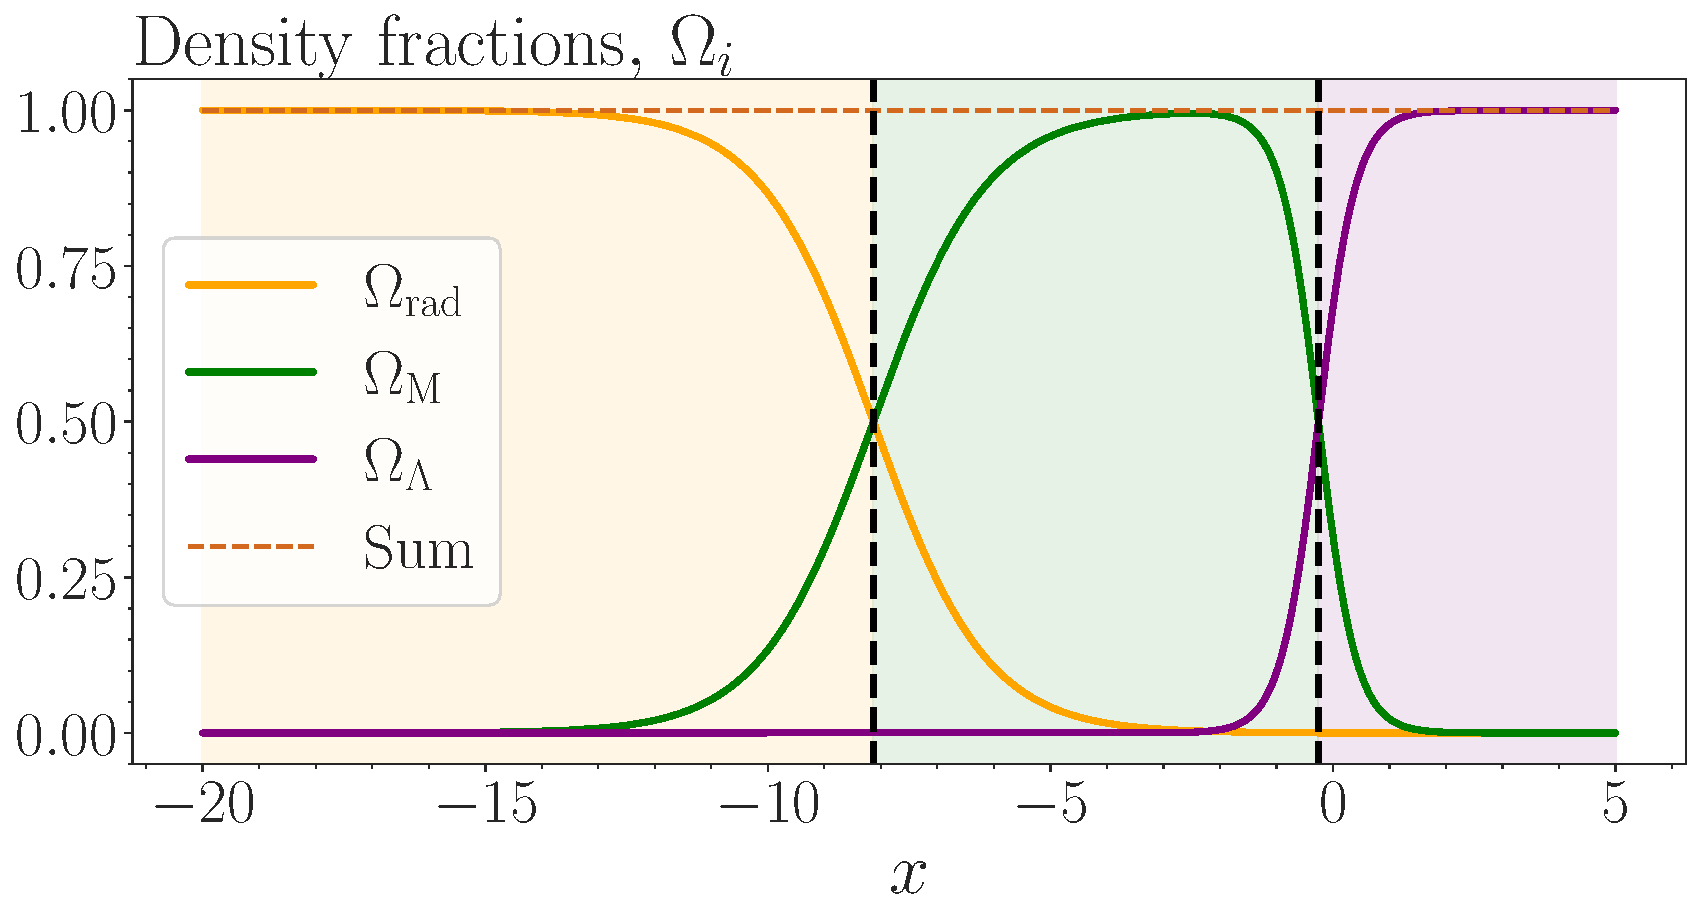
\includegraphics[width=\linewidth]{testing_omegas.pdf}
        \caption{Density fractions $\O_i$ as function of $x$. For low $x$, radiation dominates, before matter dominates and dark energy has just become the dominant energy density today $x=0$, and will continue to dominate into the future. The sum of densities sums to one across all times, as required (white dotted line). The black dotted lines are the radiation-matter equality at $x=-8.13$ and the matter-dark energy equality at $x=-0.26$, both stated in ~\cref{tab:m1:important_values}. The domination of each regime is shown as a shaded background with similar colour as its respective graph. }
        \label{fig:m1:omega_tests}
    \end{figure}
    
    \TODO{fix this}
    As explained in section ~\cref{sec:m1:theory:sanity}, we have analytical solutions for constructions of $\eta$ and $\Hp$ in the different regimes. \cref{fig:m1:eta_tests} is the sanity check for $\eta$, showing $\eta\Hp/c$ converging to finite values in the radiation and matter dominated eras (where $\alpha_{\mathrm{rad}, \mathrm{M}}>0$), and diverging towards $+\infty$ in the dark energy dominated era ($\alpha_\Lambda =-2 <0$). This is in accordance with the analytical solutions. The different regimes are shown in shaded colour. It is also worth noticing that $(\d \eta /\d x)\Hp/c$ is one for all regimes, as expected from equation ~\cref{eq:m1:theory:measures:eta_diffeq}. \TODO{to this}

    \begin{figure}
        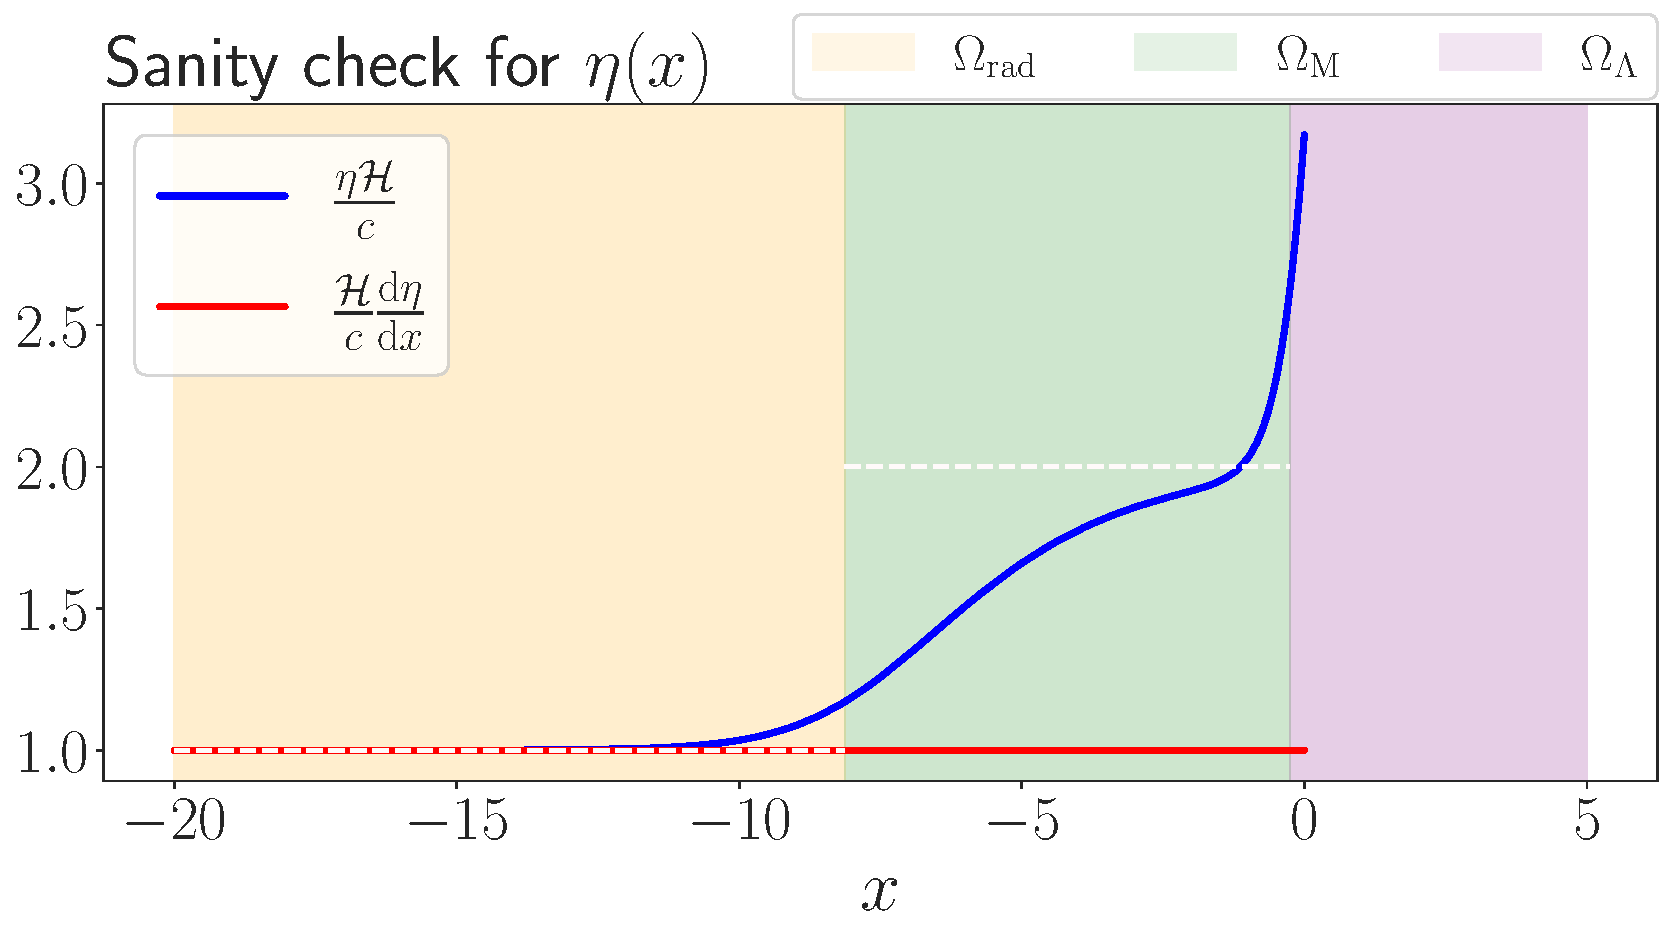
\includegraphics[width=\linewidth]{eta_test.pdf}
        \caption{Sanity check for $\eta$. $\eta\Hp/c$, in blue, is 1 in the radiation regime, 2 in the matter regime and diverging toward $+\infty$ in the dark energy regime, as expected from the analytical approximations in each regime. Remembering that this is strictly correct only in the radiation regime explains the mismatch of the brown doted line in the matter regime. $(\d \eta /\d x)\Hp/c$, in red, is 1 throughout time, as expected from ~\cref{eq:m1:theory:measures:eta_diffeq}.}
        \label{fig:m1:eta_tests}
    \end{figure}

    ~\cref{fig:m1:Hp_tests} is the sanity check confirming that our constructions of $\Hp$ and its derivatives converge to the analytical approximation in the different regimes. The second derivative, as shown in blue, takes the value of 1 in the radiation regime, 1/4 in the matter regime and 1 in the dark energy regime. Similarly, the first derivative, as shown in red, take the value -1 in the radiation regime, -1/2 in the matter regime and 1 in the dark energy regime. This is well in accordance with the analytical approximations put forth in section ~\cref{sec:m1:theory:sanity}. 

    \begin{figure}
        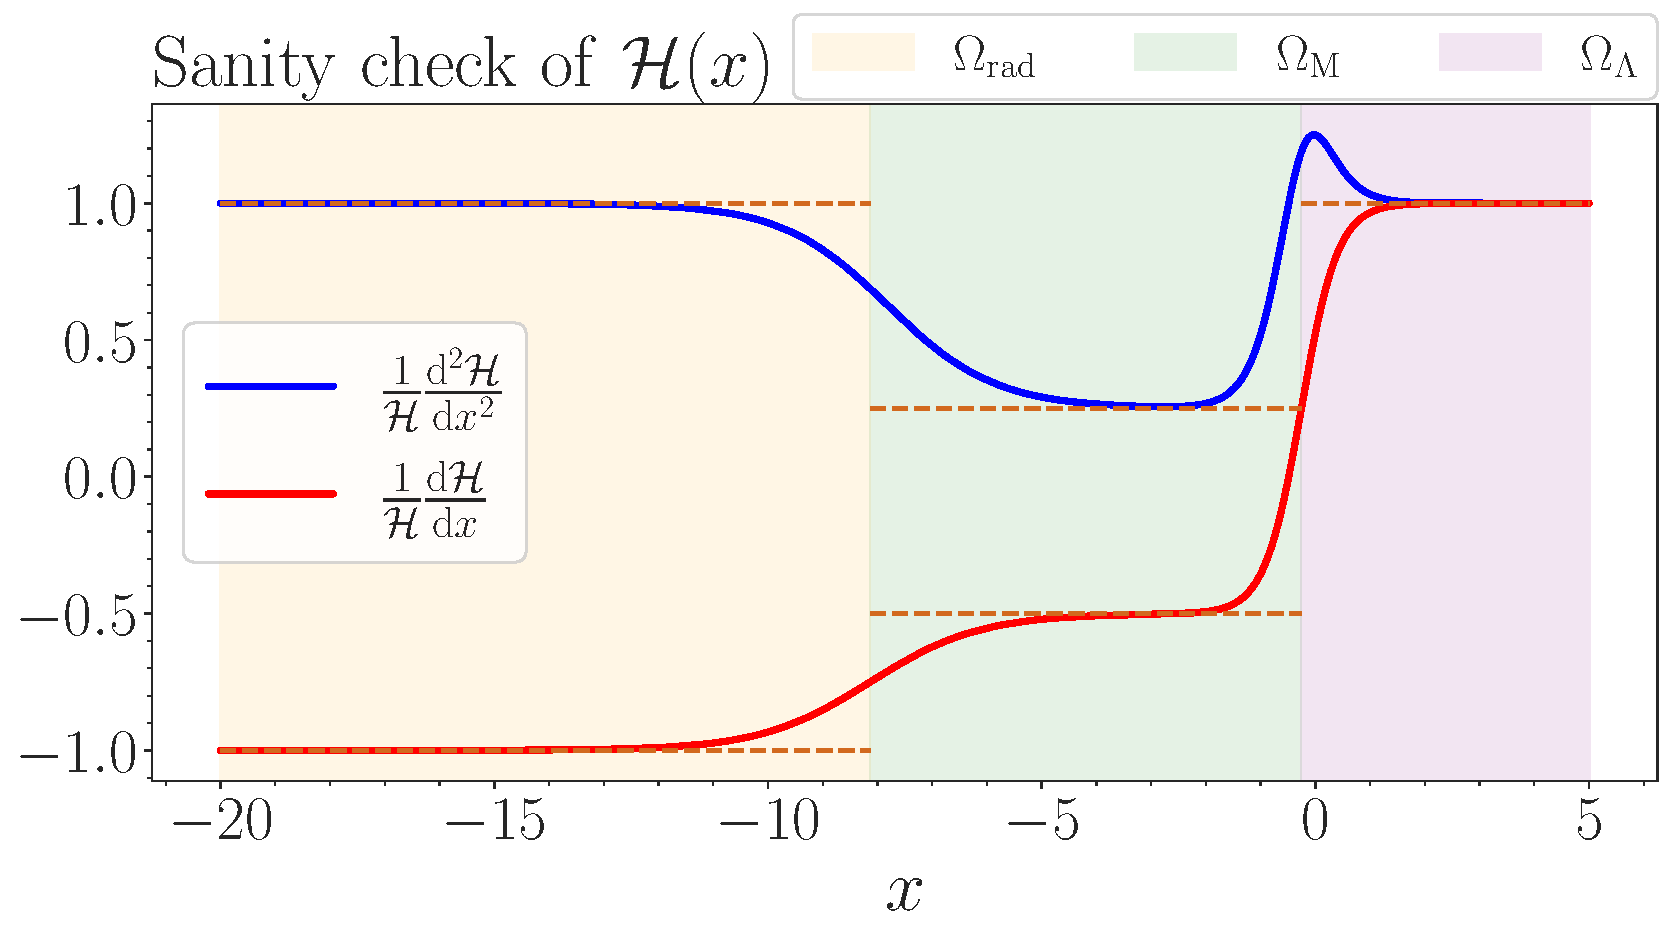
\includegraphics[width=\linewidth]{Hp_test.pdf}
        \caption{Sanity check for $\Hp$, showing that the second derivative (blue) converge to the analytical expressions shown as brown dotted lines in the different regimes. The first derivative (red) converge to its analytical values in the same regimes, which again are shown with a shaded colour.}
        \label{fig:m1:Hp_tests}
    \end{figure}

    These sanity checks are confirmations that the implementations yield the same result as the analytical approximation in the different regimes for various constructions of $\eta$ and $\Hp$ and their derivatives.
    
\subsubsection{Analysis}

    In ~\cref{sec:m1:lambdaCDM} we indicate how we can calculate the radiation-matter equality (RM-equality), matter-dark energy equality (ML-equality), when the acceleration of the universe started, the age of the universe and the conformal time today. The result is shown in ~\cref{tab:m1:important_values}. We note that the equalities is in accordance with the sanity checks, and the age of the universe today (in cosmic time) is about 13.9 Gyr. We also note that the acceleration onset is slightly before the matter-dark energy equality at $x=-0.49$ and $x=-0.26$ respectively. 
    \begin{table}
        \begin{tabular}{lrrrl}
Quantity & x & z & t [Gyr] &  \\
RM-equality  & -8.13 & 3400.33 & 0.000051 &   \\
ML-equality  & -0.26 & 0.29 & 10.378200 &   \\
Accel. start  & -0.26 & 0.29 & 10.378200 &    \\
Age of universe  & 0.00 & 0.00 & 13.857700 &   \\
Conformal time  & 0.00 & 0.00 & 46.318700 &   \\
\end{tabular}

        \caption{Important quantities in the evolution of the universe. RM stands for radiation-matter and ML for matter-dark energy.}
        \label{tab:m1:important_values}
    \end{table}

    The conformal Hubble factor, $\Hp$, is plotted against time, $x$, in ~\cref{fig:m1:conformal_hubble_factor_Hp}. It is decreasing in the radiation and matter regimes and increasing in the dark energy regime, switching signs at the acceleration onset, which is marked with a black dotted line in the figure. 
    \begin{figure}
        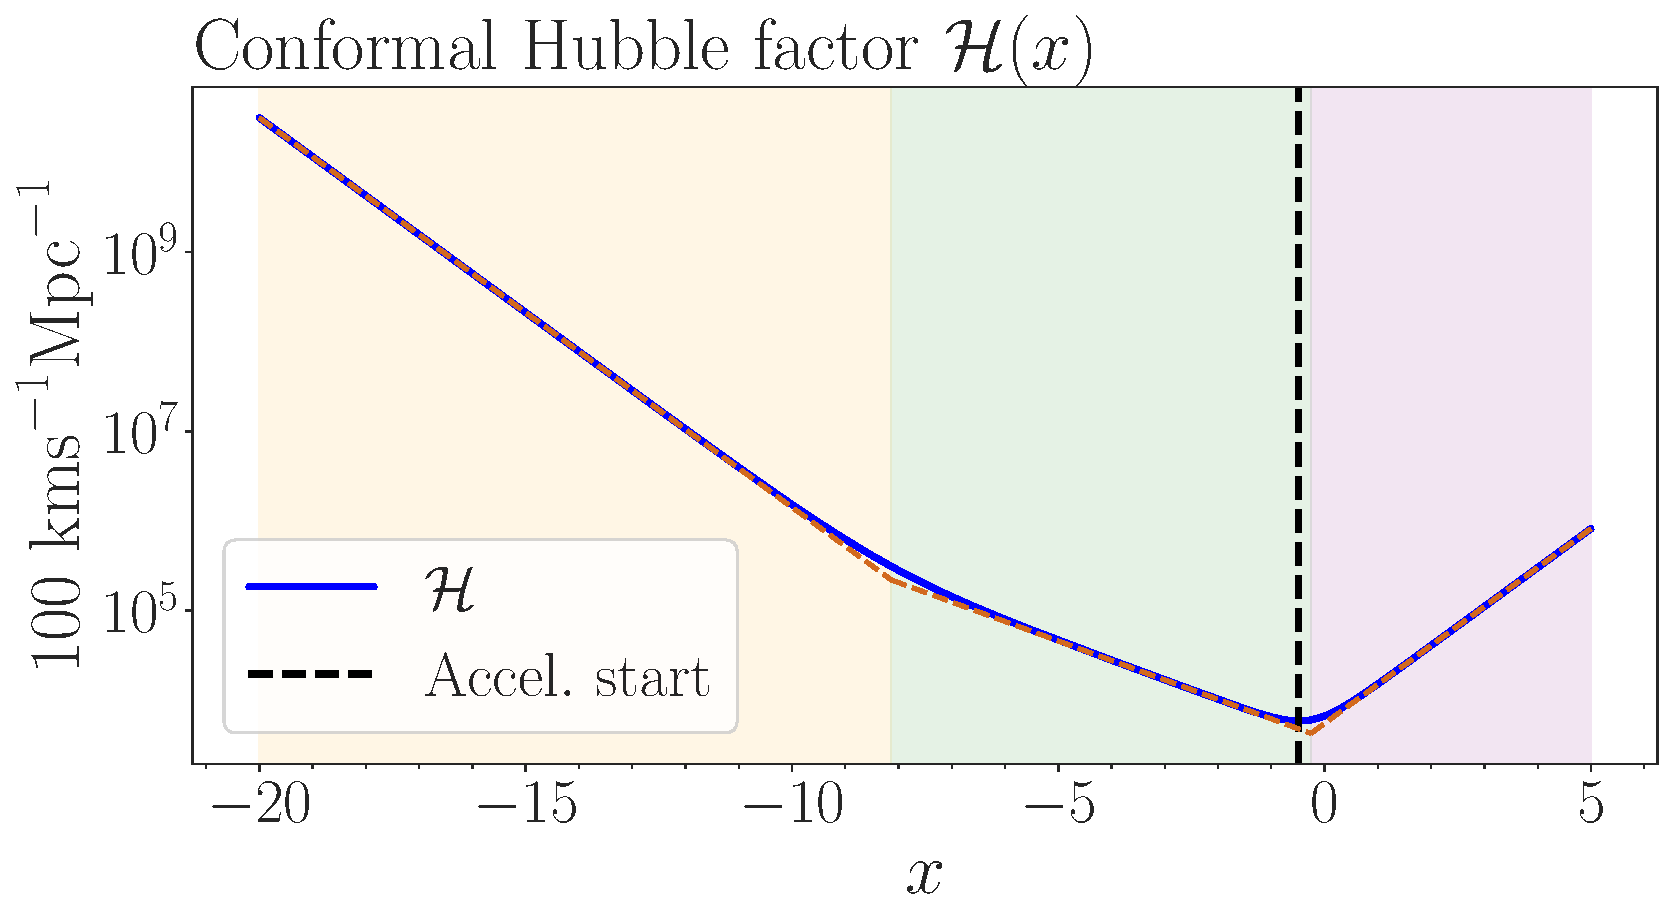
\includegraphics[width=\linewidth]{conformal_hubble_factor.pdf}
        \caption{$\Hp$ as function of $x$. It is decreasing in the radiation and matter regimes, and increasing in the dark energy regime, tightly following its analytical approximation in each regime.}
        \label{fig:m1:conformal_hubble_factor_Hp}
    \end{figure}

    ~\cref{fig:m1:cosmic_conformal_time} show the cosmic time $t$ and the conformal time $\eta/c$. The cosmic time is the age of the universe at any given time/size $x$. The low values for the cosmic time at early times suggest a rapid increase of the size of the Universe in a short cosmic time. This is supported by the conformal Hubble factor in ~\cref{fig:m1:conformal_hubble_factor_Hp} which is large for low $x$. The expansion rate of the universe decelerates until the acceleration onset, from which it accelerates. \TODO{explain $\eta$ and $t$ more}

    \begin{figure}
        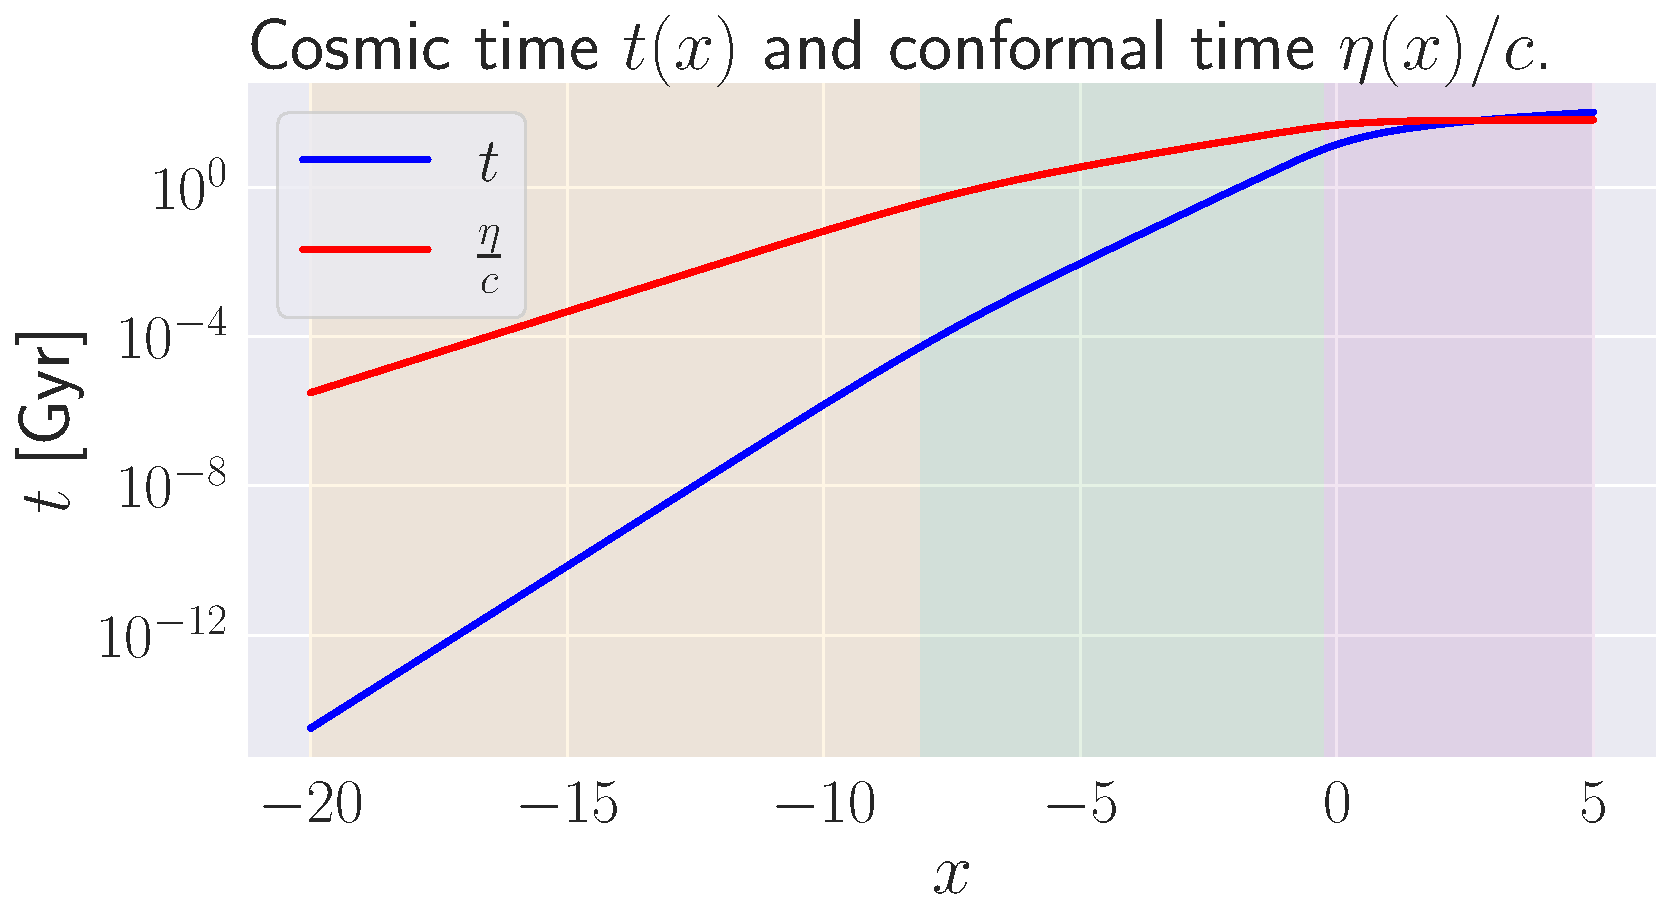
\includegraphics[width=\linewidth]{cosmic_conformal_time.pdf}
        \caption{Cosmic time (in blue) and conformal time (red). \TODO{find meaning behind this plot}.}
        \label{fig:m1:cosmic_conformal_time}
    \end{figure}

    The results of the supernova fitting, outlined in section ~\cref{sec:m1:methods:fit}, is summarised in ~\cref{tab:m1:best_fit_values}. The parameter values that maximises the likelihood (minimising) $\chi^2$ are: $h=0.702$, $\O_\mathrm{M0} = 0.259$ and $\O_{k0} = 0.274$. We also compute the posterior probability distribution function obtained from ~\cref{eq:m1:methods:fit:posterior_prob} which we have assumed to be normally distributed. From this we obtain a mean value, but also a $1\sigma$ confidence interval, which is:
    \begin{equation}\label{eq:m1:results:posterior_results}
        \begin{split}
            h &= 0.701\pm0.006 \\
            \O_\mathrm{M0} &= 0.247\pm0.110 \\
            \O_{k0} &= 0.107 \pm 0.274
        \end{split}
    \end{equation}
    \TODO{cont.}
    \begin{table}
        \begin{tabular}{l|rrr}
      & $h$ & $\O_\mathrm{M0}$ & $\O_{k0}$  \\
    \hline
    Best: $\min{\chi^2}$  & 0.702 & 0.259 & 0.067  \\
    Posterior  & 0.701 & 0.247 & 0.107   \\
    $1\sigma$ confidence  & 0.006 & 0.110 & 0.274 \\ 
    \hline
    \hline
\end{tabular}
        \caption{Best and fitted values. The best fit values are those that actually minimise the $\chi^2$-value, which consequently are the most probable values. The fitted values are obtained as the mean and standard deviations of the posterior pdfs of the parameters respectively. }
        \label{tab:m1:best_fit_values}
    \end{table}

    ~\cref{fig:m1:supernova_data} shows the supernova data as red error bars, with the predictions from the fiducial cosmology plotted above it, alongside the best fit parameter values. The quantity plotted is the luminosity distance divided by redshift, $d_L/z$ for better comparison. We notice the accordance between the two, and also note that the $x$-axis in this plot is the redshift $z$ instead of the logarithm of the scale factor. This means that earlier times are to the right in the plot (high redshift), as opposed to the other plots. 

    \begin{figure}
        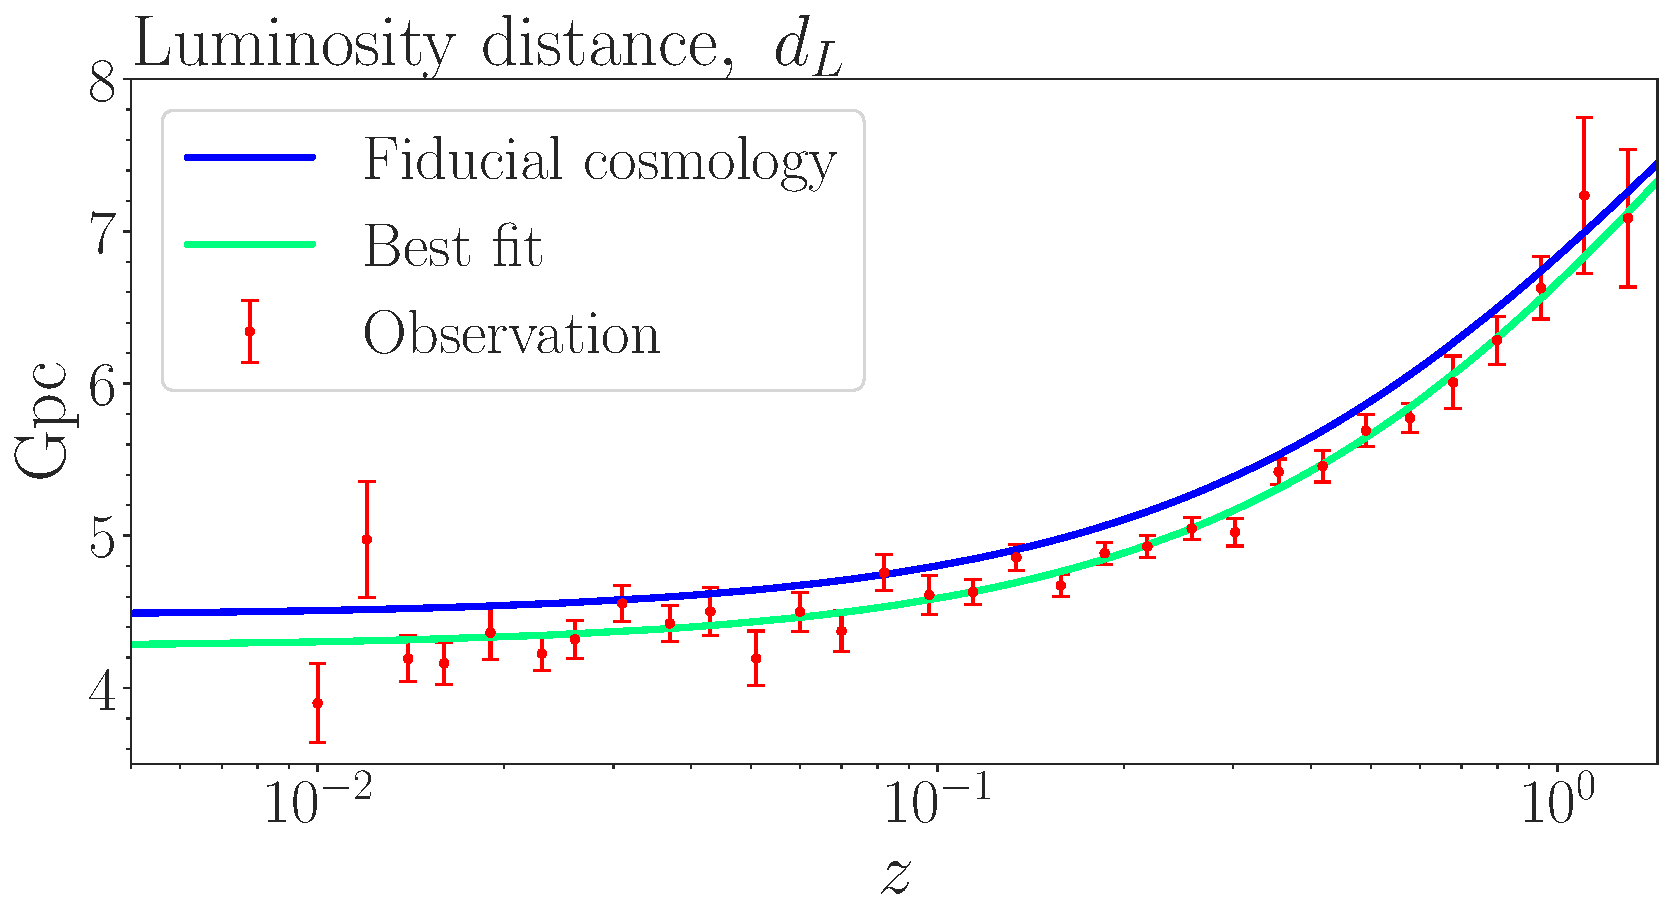
\includegraphics[width=\linewidth]{supernova_data.pdf}
        \caption{The luminosity distance predicted using the fiducial cosmology in blue, against observations of actual supernovas in red (or rather the confidence interval of the observations). The green line is found from computing the luminosity distance using a cosmology of the best fit parameters from the supernova fitting; $h=0.702, \O_\mathrm{b0} = 0.05, \O_\mathrm{CDM0} = 0.209, \O_\mathrm{k}=0.067, N_\mathrm{eff}=3.046, T_\mathrm{CMB}=2.7255 \text{K}$. Notice the $x$-axis is now the redshift $z=e^x-1$.}
        \label{fig:m1:supernova_data}
    \end{figure}

    \begin{figure}
        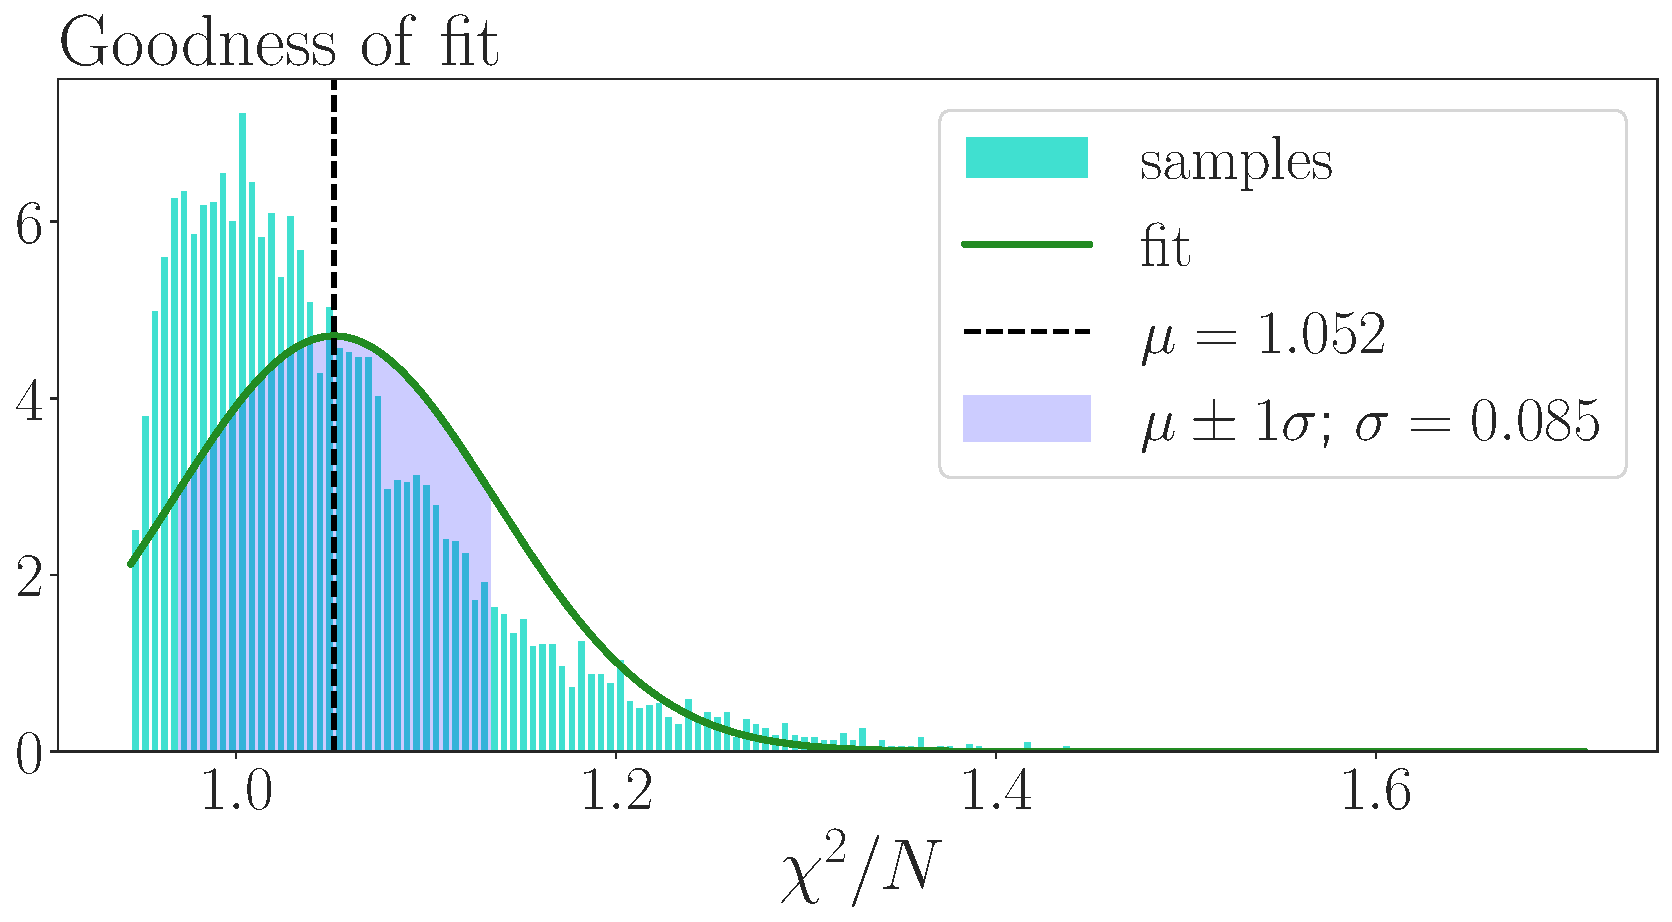
\includegraphics[width=\linewidth]{goodnes_of_fit.pdf}
        \caption{Goodness of fit}
        \label{fig:m1:goodness_of_fit}
    \end{figure}

    \cref{fig:m1:omega_planes} shows the $\chi^2$-values found from \cref{eq:m1:chi2_test_def}, to 1$\sigma$ accuracy. The black dotted line represent a flat universe, where the matter and dark energy are the main constituents of the universe. The supernova data originate in close temporal proximity to us, we thus assume that the contribution from the radiation density is negligible for making constraints on $\O_\mathrm{M}$ and $\O_\Lambda$ today. 

    \begin{figure}
        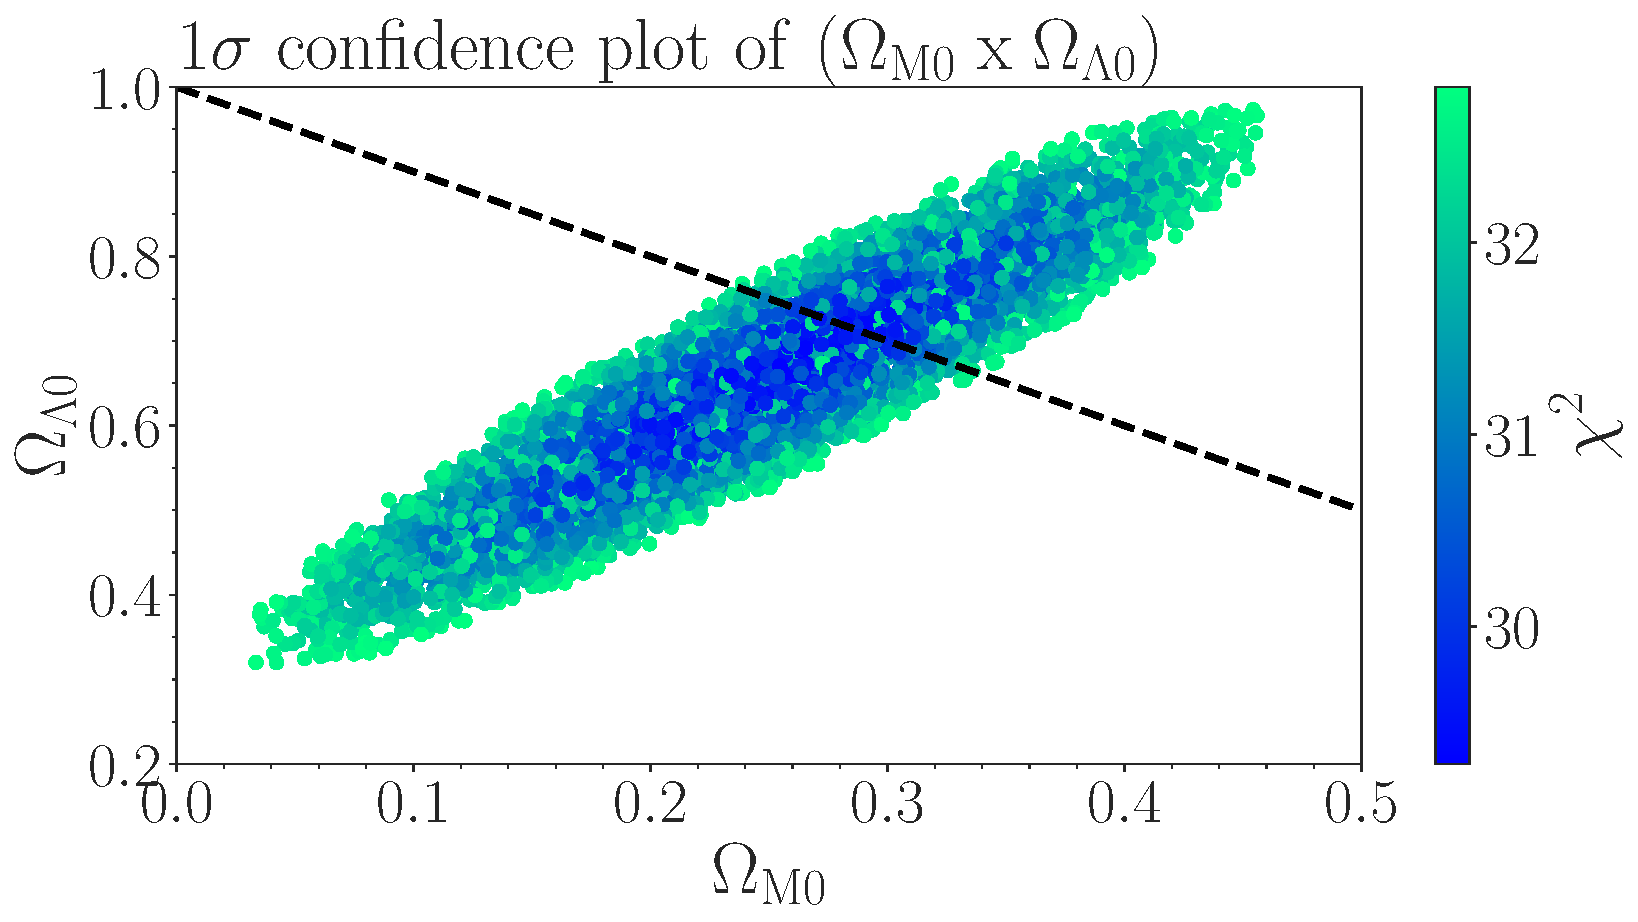
\includegraphics[width=\linewidth]{omega_plane.pdf}
        \caption{Scatter plot showing the $chi^2$-error of the luminosity distance $d_L$ between the observed values and the prediction, as function of $\O_\mathrm{M}$ and $\O_\Lambda$. The data shown is within $1\sigma$ (standard deviation). The black dotted line signifies a flat universe. }
        \label{fig:m1:omega_planes}
    \end{figure}

    The MCMC method allow us to make a posterior probability distribution of the parameters in question. \cref{fig:m1:posterior_pdf_H0} the distribution of the Hubble factor $H_0$ constructed from the sampled values of $h$. The actual samples are shown in green and the corresponding fitted probability distribution in blue. 


    \begin{figure}
        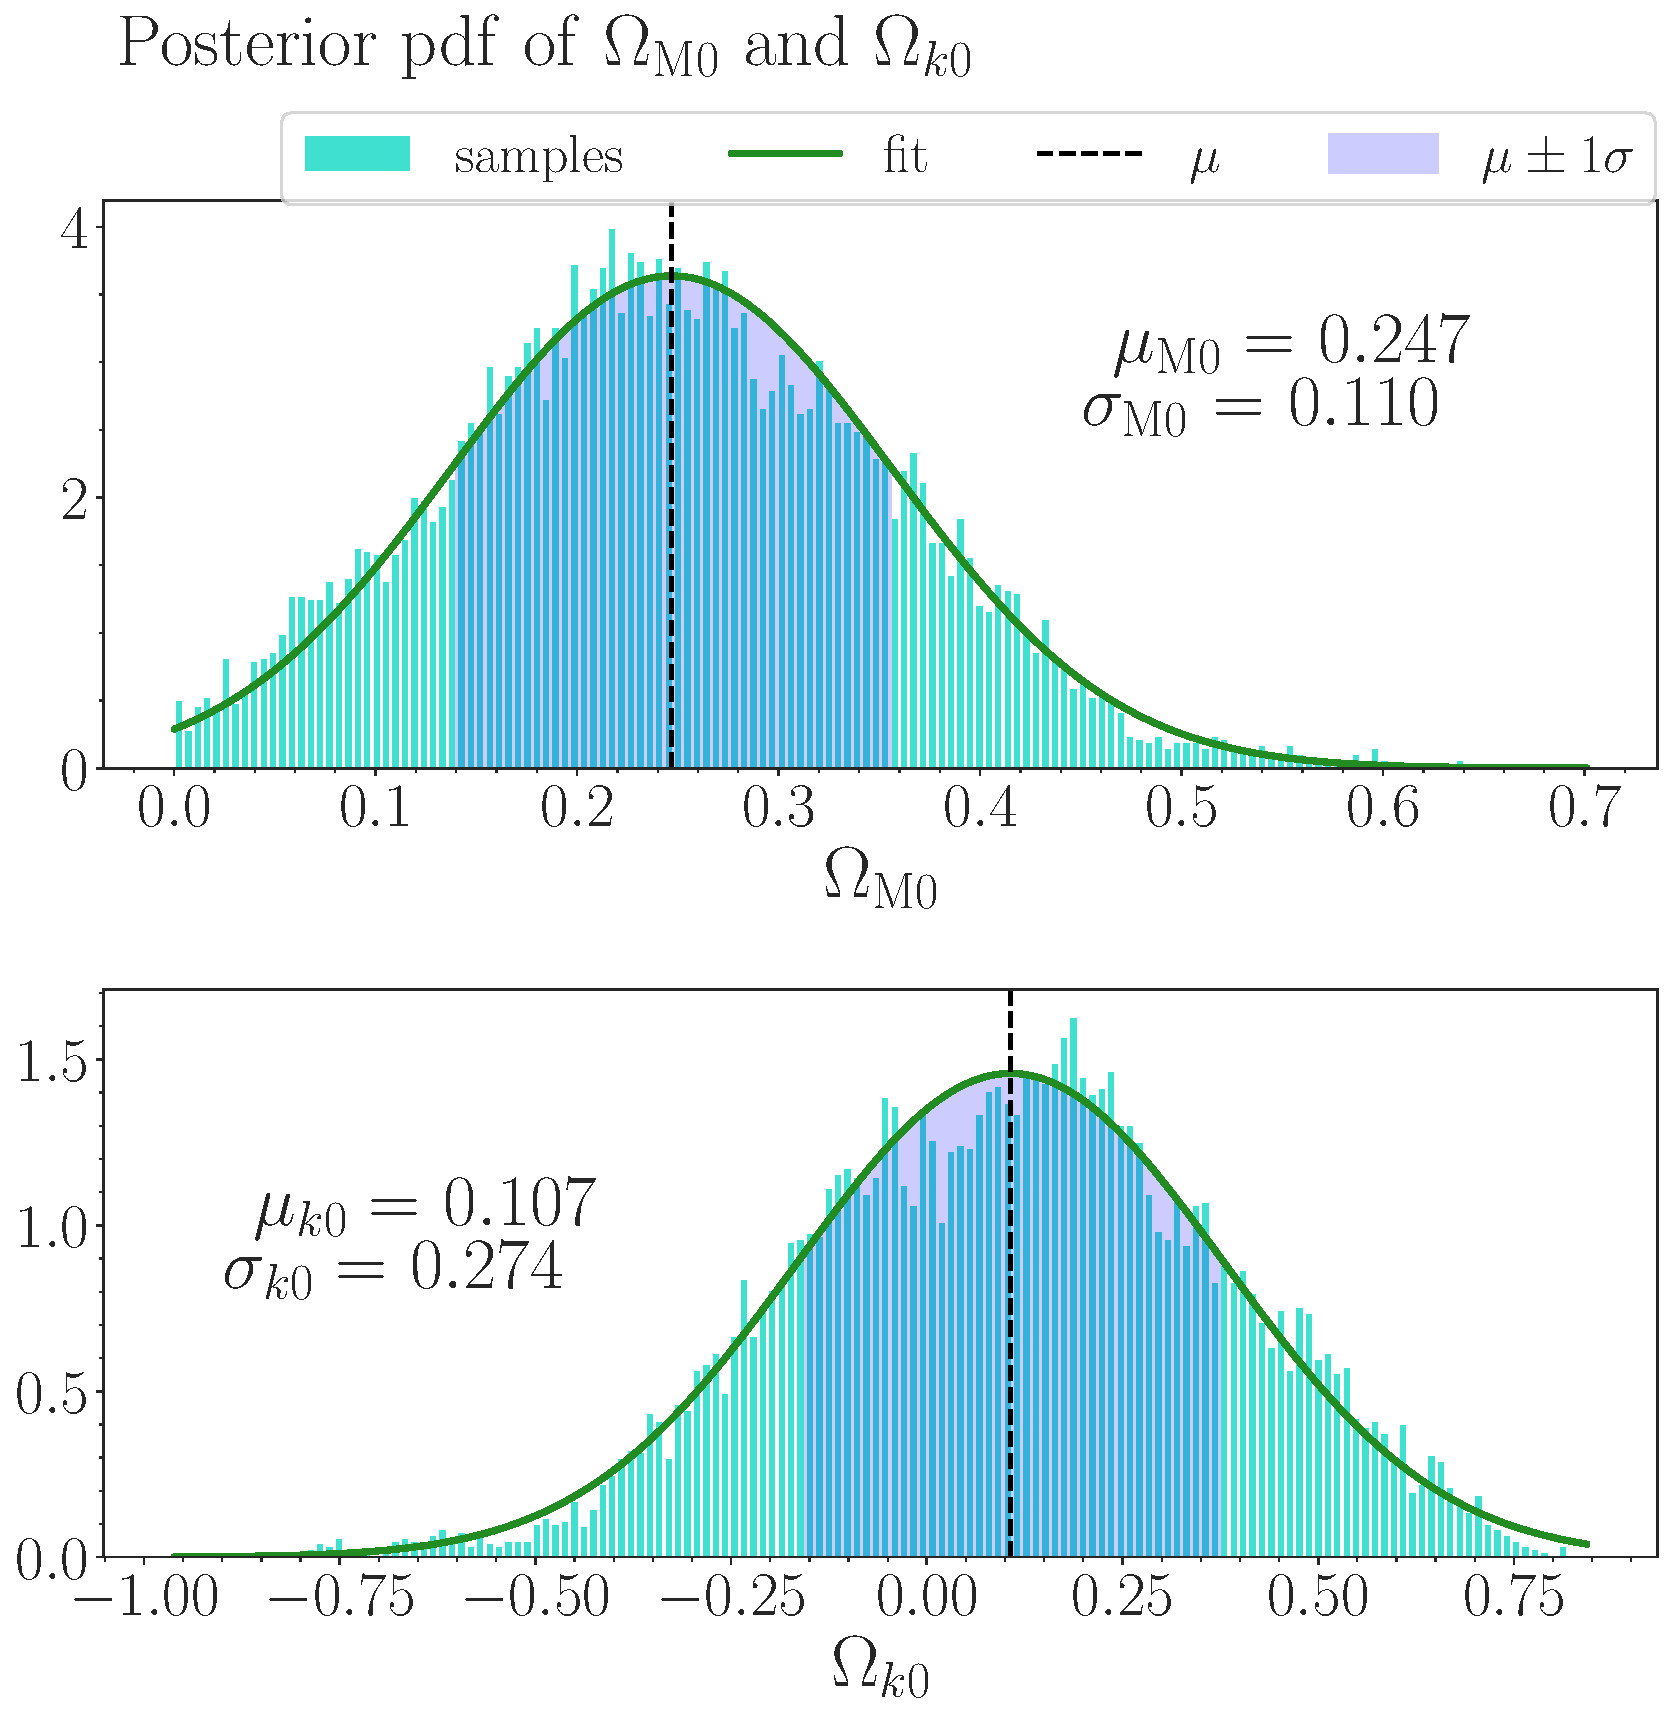
\includegraphics[width=\linewidth]{probs_M_K.pdf}
        \caption{Posterior probability distributions (pdfs) of $\O_mathrm{M}$ and $\O_\mathrm{k}$ as result of the MCMC sampling. The samples as shown in turquoise and the constructed pdfs in green. The mean $\mu$ is shown as a black dotted line, with the $1\sigma$ confidence interval in shaded blue ($\mu\pm 1\sigma$)}
        \label{fig:m1:posterior_pdf_omega_m_k}
    \end{figure}

    \begin{figure}
        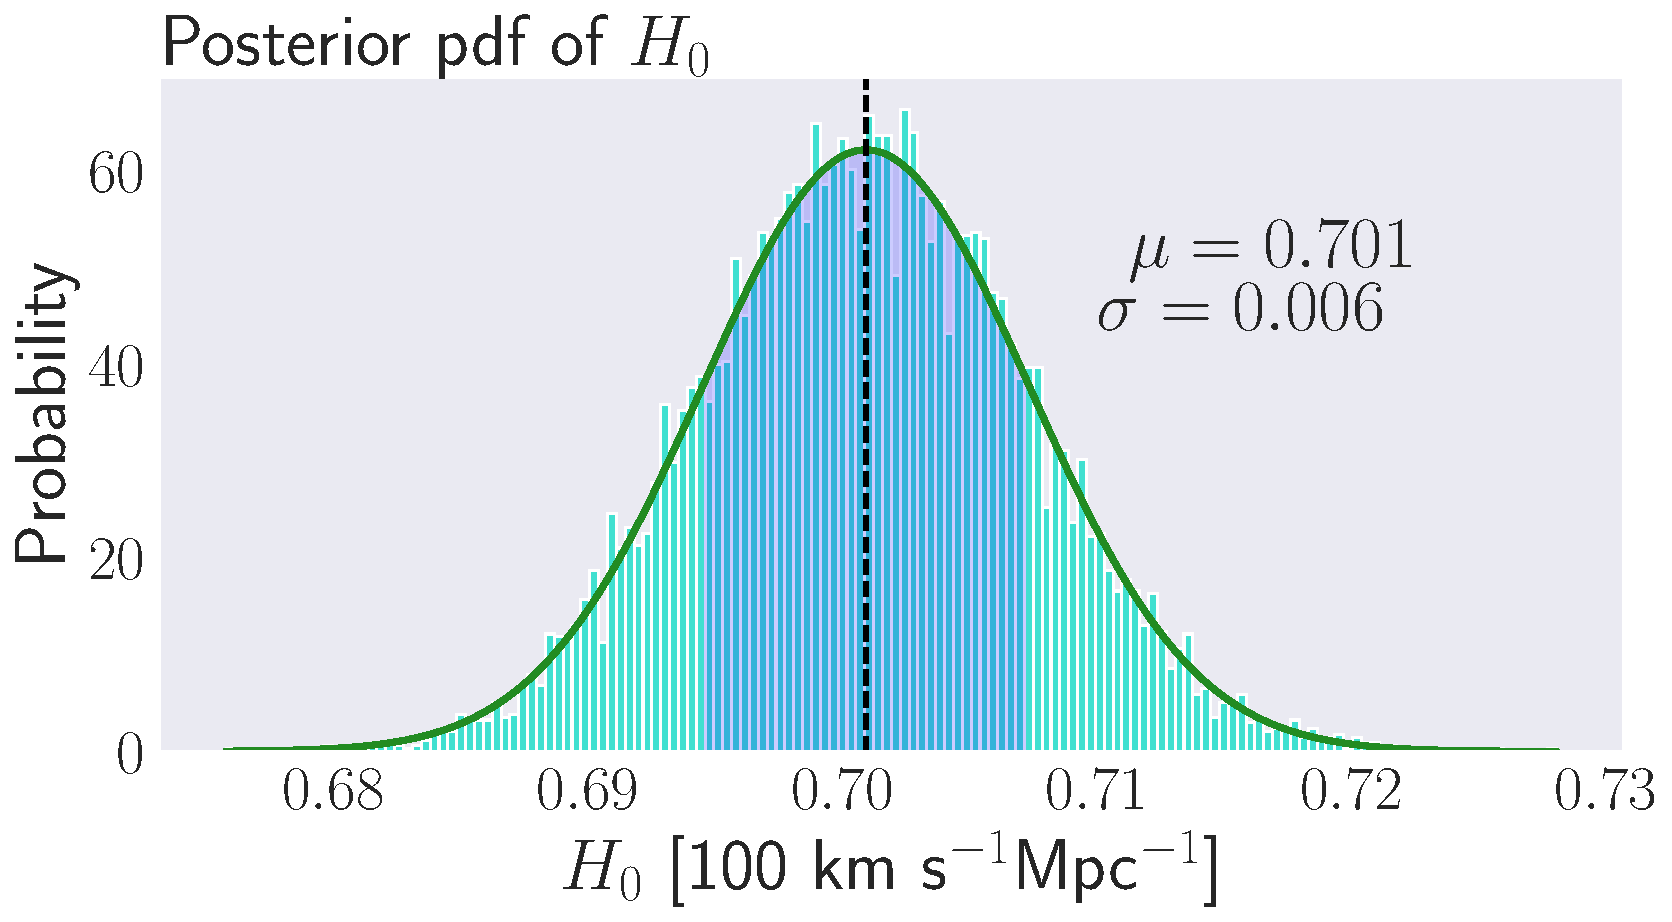
\includegraphics[width=\linewidth]{posterior_pdf.pdf}
        \caption{Posterior probability distribution (pdf) of $H_0$ as result of the MCMC sampling.}
        \label{fig:m1:posterior_pdf_H0}
    \end{figure}

